% !TEX root = ../thesis.tex

\chapter{Use Cases and Evaluation} \label{evaluation}

In this section, we first walk through some example use cases for Intertext. It is worth noting that at the time of writing, only the Intertext web client is fully implemented. Therefore some of the examples mentioned in this section are given with our future plans in mind. Moreover, some of the use cases are of things that could theoretically and practically be built on top of the Intertext ecosystem, not by us but by the community. 

Later on, we will explain the evaluation process. To execute the evaluation, we have built \dquote{RecipeApp}, a sample Intertext application where users can sign up, log in, add recipes, and browse recipes other users added. It was specifically built to showcase all the functionality that Intertext offers. While the use cases section is intended as example use cases for the users, this section could be thought of an example use case scenario for developers, giving ideas on how an Intertext application can be built. In this section, we will first talk about RecipeApp; how it is built and how it works under the hood. Then, we will discuss the user evaluation process and share the results.

\section{Use Cases}

\subsection{Back-end Developer}

Harry is a software engineer. He recently graduated from college, and started his career as a backend engineer. While work is busy, he is still interested in working on an idea he had in college on the side. Without losing much time, he gets to work. His most important constraint is that he has little to no budget, so he designs a low-cost scaleable serverless architecture and starts coding. After a few months of hard work, he finishes the backend portion of his application. He spins up an instance on his favourite cloud provider, he is able to utilise the generous free-tier and the free credits offered by the provider to scale up to thousands if not millions of users at almost no cost. 

Then he realises that he still needs a front-end for his application. Not only does he need a web presence, he also needs a mobile app to meet his users' needs. He has no front-end experience, nor does he have the budget to outsource the task or time to learn. So he decides to make his product an Intertext application. He makes use of the existing backend to create an additional endpoint that serves the front-end in IUIDL, and in a matter of days, he finishes the fully functional front-end and is ready for the beta launch. With minimal effort, he was not only able to obtain web and mobile presence, his product supported all other Intertext clients as well.

\subsection{John's Old Parents}

John regularly visits his old parents. A few visits back, he brought with him a gift, a computer, as an effort to introduce them to technology. He helped to set it up, and gave them a walk through on how to use it. He thought them how to perform tasks such as online banking, checking the news, checking the weather, using social media and so on. 

On his last visit, his parents mentioned that they were having some problems with the computer. He turns it on to assist them, only to find that the computer is filled with of harmful malware and games/apps that were clearly downloaded out of intention. He asks them how it happened, and they told him that it all started when they clicked \dquote{OK} on a popup that appeared on one of the websites. The default home page was replaced, new harmful browser extensions were installed, the computer became slow and was nearly unusable. So he formats the computer, and installs the Intertext desktop client. He teaches them about how to use the Intertext apps for their favourite news websites, bank, social media, and other services they use. He tells them that they can enjoy a clean, consistent and safe experience, with no intrusive ads, harmful software, trackers, background scripts and so on. 

Another thing that he notices is that they struggle to see the screen and read text very well. Also since they are not accustomed to using a computer mouse, their mouse movement is unstable and clicks are inaccurate. They often misclick on things they did not intent to click, causing them to navigate away to another page and miss context, which gets them confused and frustrated. To combat these issues, he creates a custom theme for them. He makes the text bigger and bolder, buttons and links larger and harder to miss. Thanks to Intertext, his parents are able to use web more comfortably and confidently.

\subsection{New Device On The Market}

X, Inc is a promising startup working on a new kind of wearable device. This device can perform all functions of a mobile phone; make calls, send messages, take pictures, browse the internet and so on. It has the potential to replace mobile devices for some people, however it has a downside that holds it back: it has no application support. There are no third party applications built that can run on their device natively. It do have a web browser; but due to the nature of this device, browsing web applications on its screen is very uncomfortable. They realise that their potential customers don't want to leave their phone behind when they can't use their day-to-day applications properly. As a solution, they decide to make use of the open-source Intertext ecosystem. They build an Intertext client that runs natively on their device and renders IUIDL optimised for its input/output (I/O) constraints. With their new Intertext client, they now have access to the entirety of the Intertext applications. They are now set to release their product with no compromises and full confidence.

\subsection{Clients For Special Needs}

Sally is a developer working on an initiative for creating software that makes it possible for people with disabilities that cannot use a mouse or a keyboard to be able to use a computer. They experiment with different input/output methods such as retina tracking, voice interfaces, neural-control interfaces and so on. With their software, users can chose the I/O method that best suits them to use their computer. However in most cases, it is very hard to use a software that was built with no accessibility features. So she decides to use Intertext to improve this process. Knowing that it is guaranteed that all Intertext applications are accessible by default, she builds the software to take advantage of the Intertext web client. Moreover, for other I/O methods they experiment with that needs support for a custom/specific GUI, she creates individual Intertext applications.

\subsection{No-Code Universal Application Builder}

With the increasing popularity of the no-code movement, more and more companies are looking for code-free solutions to problems that used to require programming skills. Y, Inc is one of these companies. They want to invest in a platform that allows everyone to create applications for different devices and environments. They are also aware of their constraints. They know that a one-size-fits-all solution is extremely hard to build, as every platform runs on different technologies, they have different layout systems, different runtime and so on. And then they discover Intertext. They realise how easy it is to create a tool to build Intertext applications, since all there is to do is to generate simple IUIDL code in XML syntax. Also, the logic that front-end applications needs to perform such as making requests and state management are also operated through the same syntax. Moreover, the applications generated by the tool would be universal, that is, it could run on every platform that Intertext has a client for and will have a client for in the future. They create a service that allows users to build and serve Intertext applications with ease, without writing a single line of code. This makes it possible for hobbyists to put together a simple interface without prior programming knowledge.

 
\section{RecipeApp}

While building RecipeApp, we wanted to keep things simple as its purpose is demonstration of Intertext, and we still tried our best to stay true to a real wold scenario of building applications. We created a real backend application that serves IUIDL through a restful endpoint. We used Node.js as the server-side technology, and express framework to create the endpoints. As for the database, we created a fake api that resembles a real Object Relation Mapping (ORM), which stores data in the memory.

In a real-world front-end application, it is very common to create UI elements as reusable components. This is no different for Intertext application, in a real world scenario it is clear that the best practice would be to create components out of commonly repeating UI patterns, and use instances of those components rather than duplicating IUIDL code. While creating components and reusing them on the front-end is much simpler as there are many front-end frameworks/libraries like React that enables building UI declaratively and eliminates the need for imperative manipulations, in order to do this with ease on the backend side, we needed a templating engine. For this purposes, we used the Handlebars, a popular template engine for Node.js applications.

For the time being, only the web client of Intertext is fully implemented. Therefore, the demonstration will be made on the web client and all respective screenshots are from there. However once the other clients are ready, they will be able consume the same application as it is.

\subsection{Introduction}

\begin{figure}[htb]
  \centering
  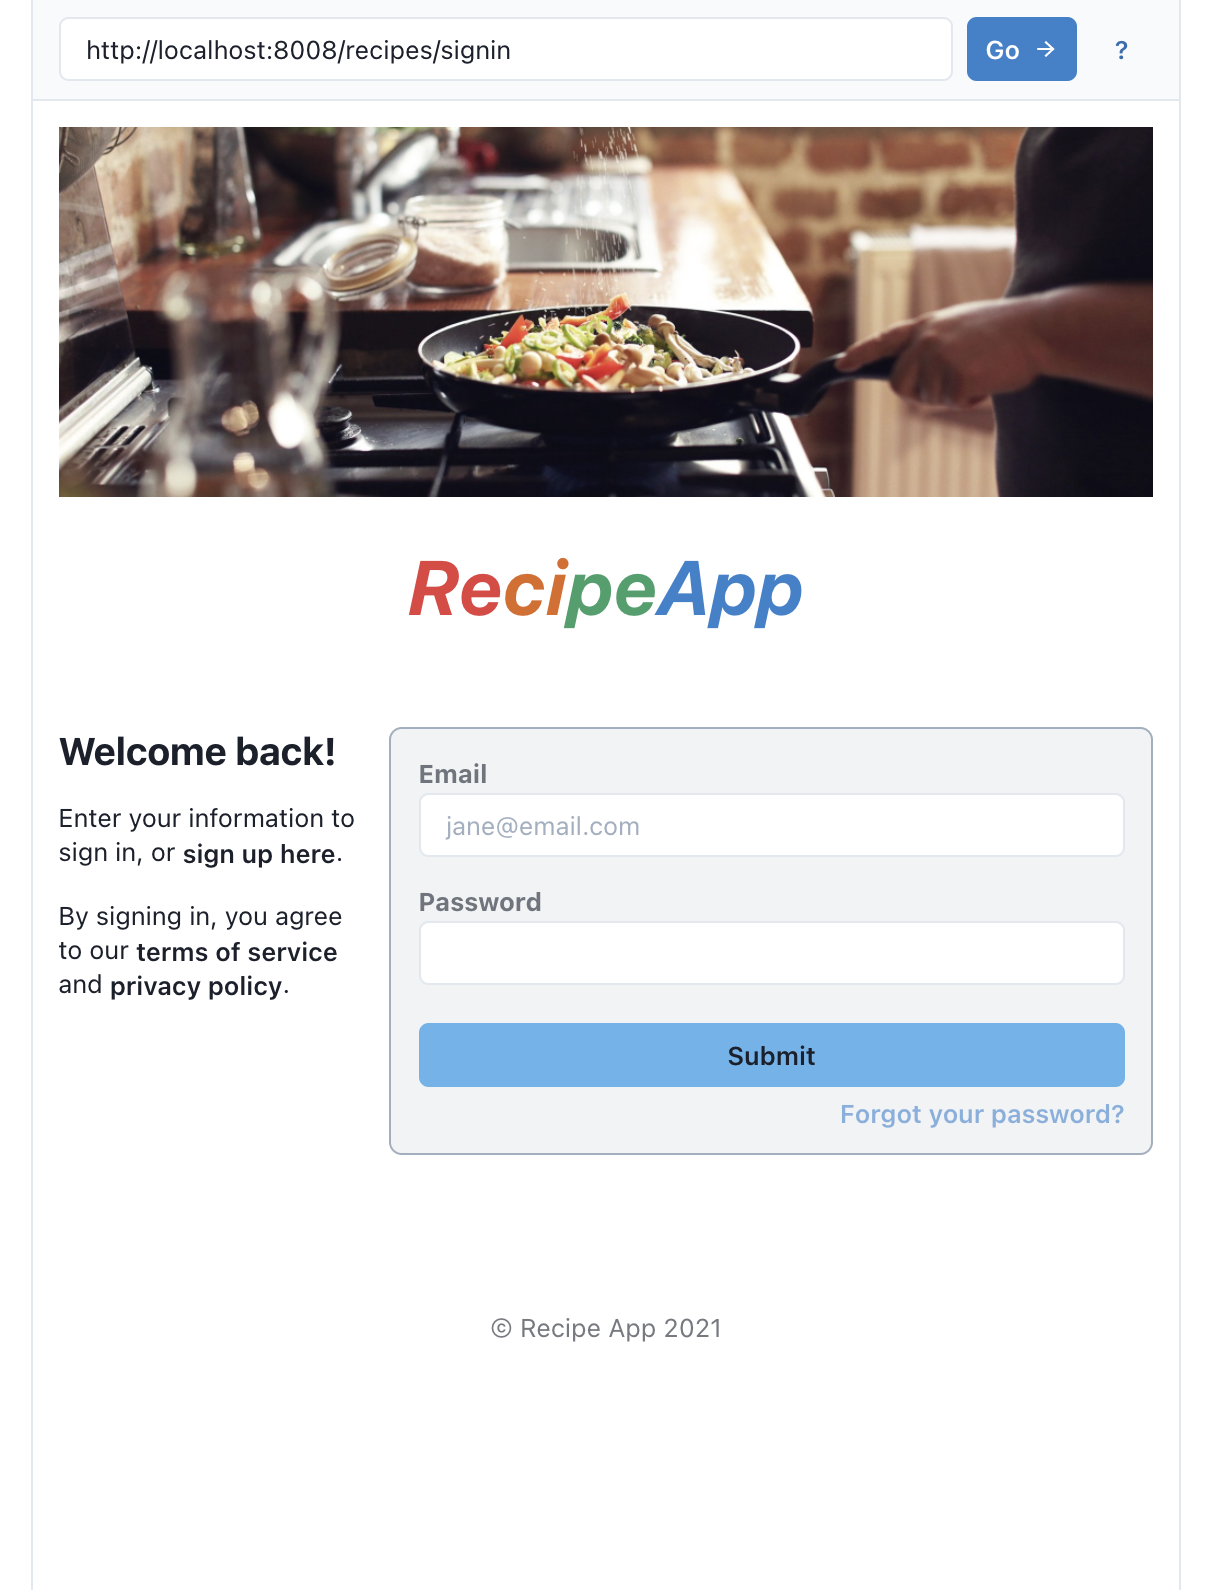
\includegraphics[width=6.2cm]{thesis/paper/images/rec_signin.png}
  \,
  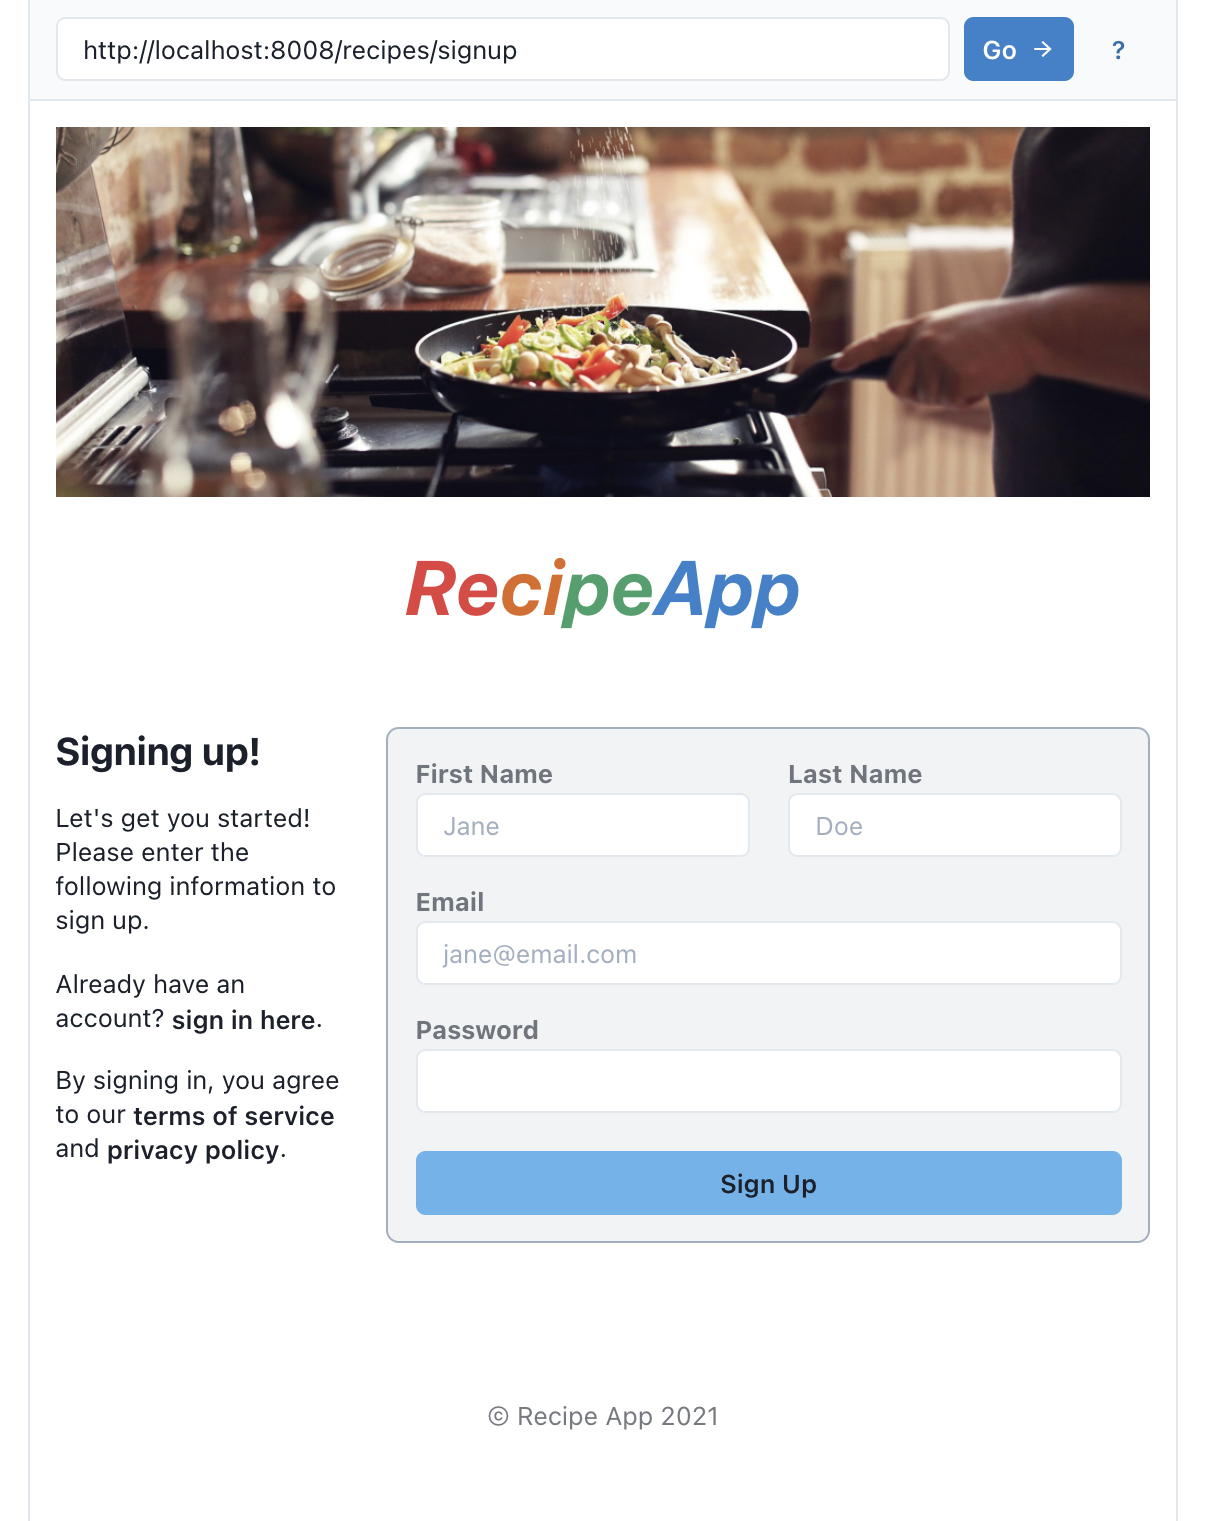
\includegraphics[width=6.2cm]{thesis/paper/images/res_signup.png}
  \caption{RecipeApp Sign In/Sign Up screens}%
  \label{fig:rec_signin_signup}%
\end{figure}

First, a user visits the URL the RecipeApp is served from via the address bar above. In figure~\ref{fig:rec_signin_signup} the example server runs on \texttt{http://localhost:3000} and the endpoint RecipeApp is served from is \texttt{/recipes}. If user is not already signed in, they will be redirected to \texttt{/recipes/signin}. After signing in from this screen, they will be redirected back to the application. If they were visiting a particular URL such as \texttt{/recipes/new} or \texttt{/recipes/3} before they got redirected to the sign in screen, they will be redirected back to that screen after signing in. Once they are signed in, they will be presented with the recipe list. The recipe list has two view options, grid view and list view, which user can chose between. The view selection will persist across sessions. Moreover, the list features a search bar, which can be used to search recipes by keywords. On each recipe item, there difficulty and time it takes to prepare the recipe is displayed along with an image. From the top navigation, user can click on the Add Recipe button to go to the insert page. From there, they can insert their own recipe.

\subsection{Authentication}

Before the authentication, the first thing to understand is how we implemented the redirection system. The redirect screen, which can be seen in Figure~\ref{fig:rec_redirect}, is essentially an handlebars template that can be rendered with some parameters and can be used for different purposes. There are two essential functions of this screen; it instructs Intertext client to store some data, and to redirect user to another endpoint. The parameters change based on the user case.

\begin{figure}[htb]
  \centering
  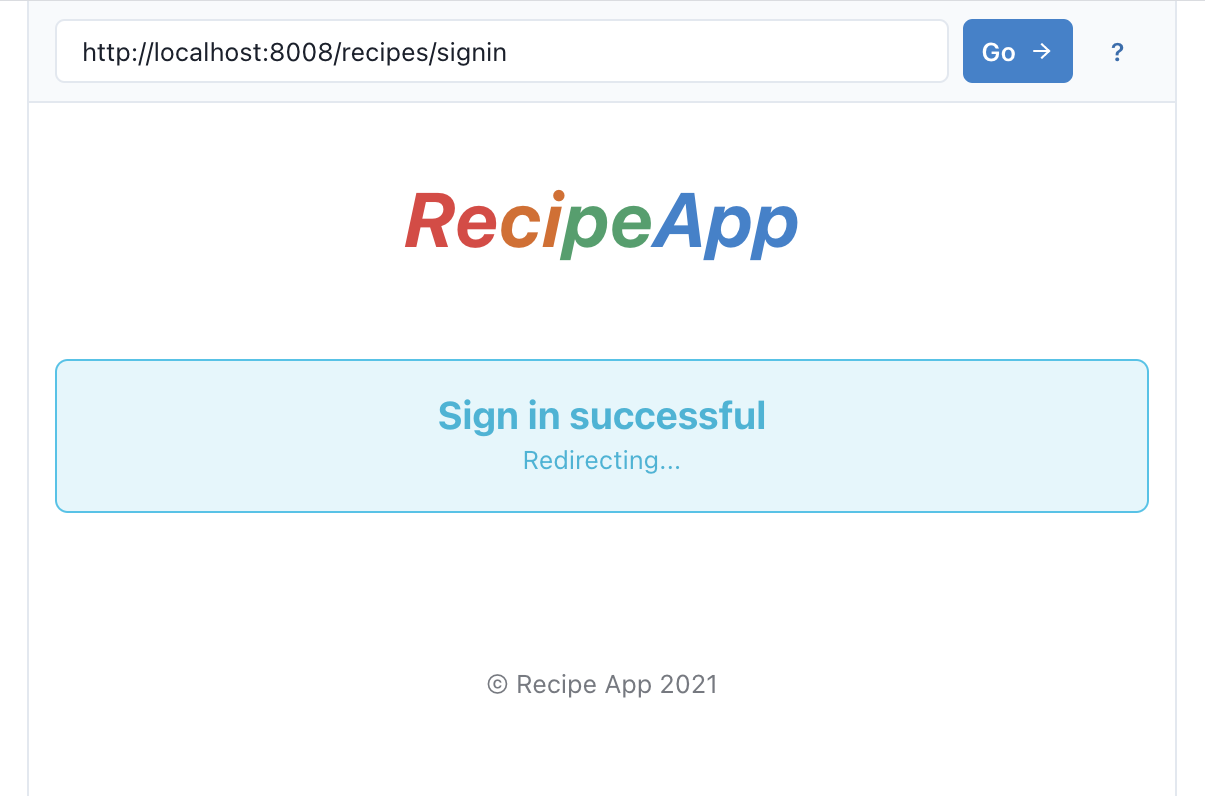
\includegraphics[width=12.4cm]{thesis/paper/images/rec_redirect.png}
  \caption{Redirect screen}%
  \label{fig:rec_redirect}%
\end{figure}

As we established before, Intertext clients pass on the application state along with every single request. When user visits the application URL, the server receives the persisted state, which is where the user token is expected to be if the user is logged in. When a user lands on any page of RecipeApp that is behind the authentication wall, the server checks the presence of \texttt{token} in request body, and if it is not present, it renders the redirect screen as shown in Figure~\ref{fig:token_capture}. 

\begin{figure}[htb]
\begin{minipage}{\linewidth}
\begin{lstlisting}[language=javascript]
const token = get(req, "body.persist.token");
if (!token) {
  res.render(view("redirect"), { ... });
} else {
  res.render(view("home"), { ... });
}
\end{lstlisting}
\end{minipage}
\caption{How token is captured on the backend}%
\label{fig:token_capture}%
\end{figure}

The redirect screen does two things: it instructs the client to store a variable called \texttt{auth-callback} which holds the URL that user is at, and it instructs the Intertext client to navigate to the \texttt{/signin} endpoint. Intertext clients does these two things, and redirects user to the \texttt{/signin} endpoint, triggering another request to the backend. The \texttt{/signin} endpoint on the backend renders the sign in form. After user submits the form with their credentials, another request to the \texttt{/signin} endpoint is made, but this time with the credentials. The backend then checks the credentials, and if it is a successful login, it once again renders the redirect screen. The redirect screen again performs two tasks: first it instructs the Intertext client to store the \texttt{token} to the persisted storage. Then, if the \texttt{auth-callback} variable is present in the request body of the request made to the \texttt{/signin} endpoint (which is where the URL user was redirected to the sign in endpoint from is stored at), it instructs the Intertext client to redirect back to that endpoint, otherwise it redirects to the home screen.

\subsection{Recipe List}

The recipes view features a list of the recipes. As seen in in Figure~\ref{fig:rec_recipe_list}, it has several components: recipe title, description, difficulty and time to cook details that are displayed in tags, and a read more button to navigate to the recipe page. The difficulty tags are made of the \texttt{block} component, and they use intents to hint the difficulty of the recipe. The view has two display options, a list view and a grid view. It also has a search input to search recipes.

\begin{figure}[htb]
  \centering
  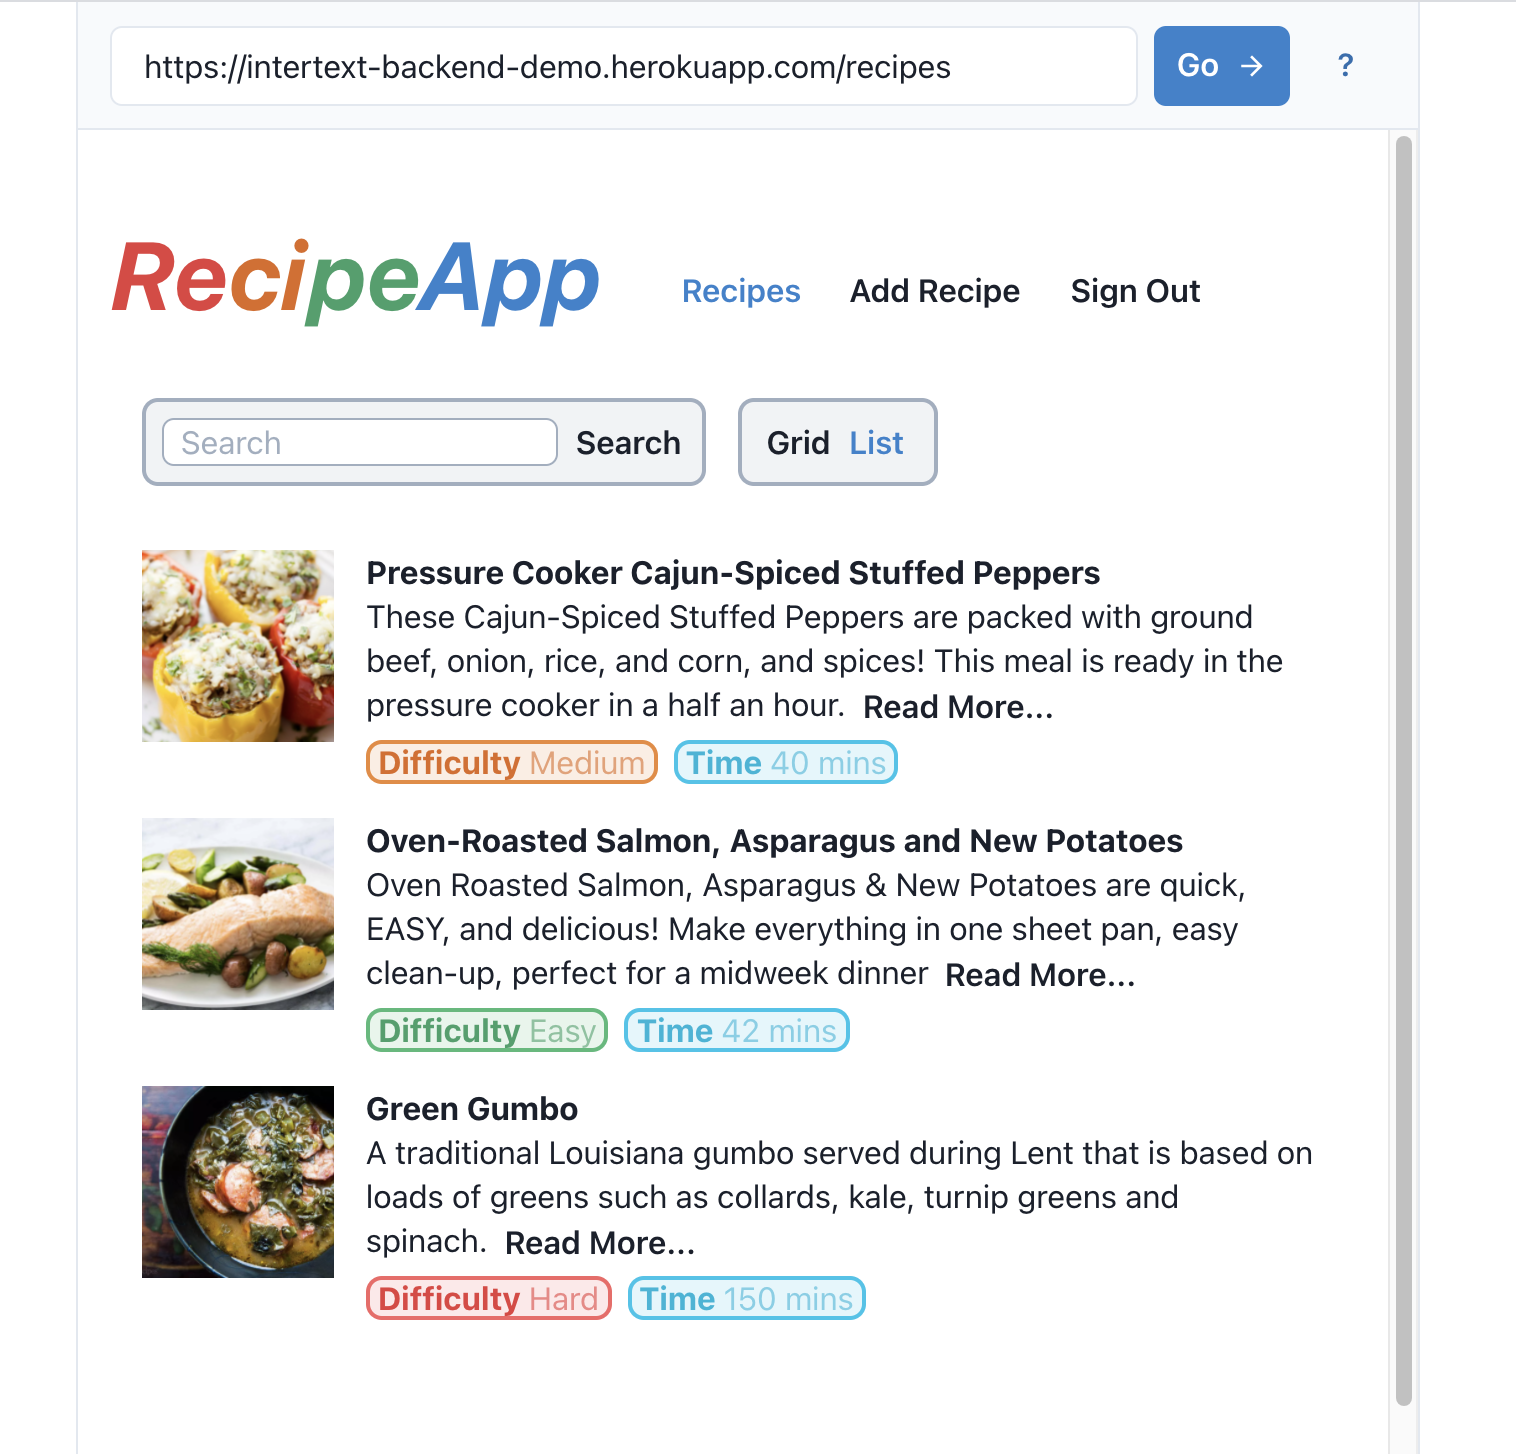
\includegraphics[width=6.2cm]{thesis/paper/images/recipe_list.png}
  \,
  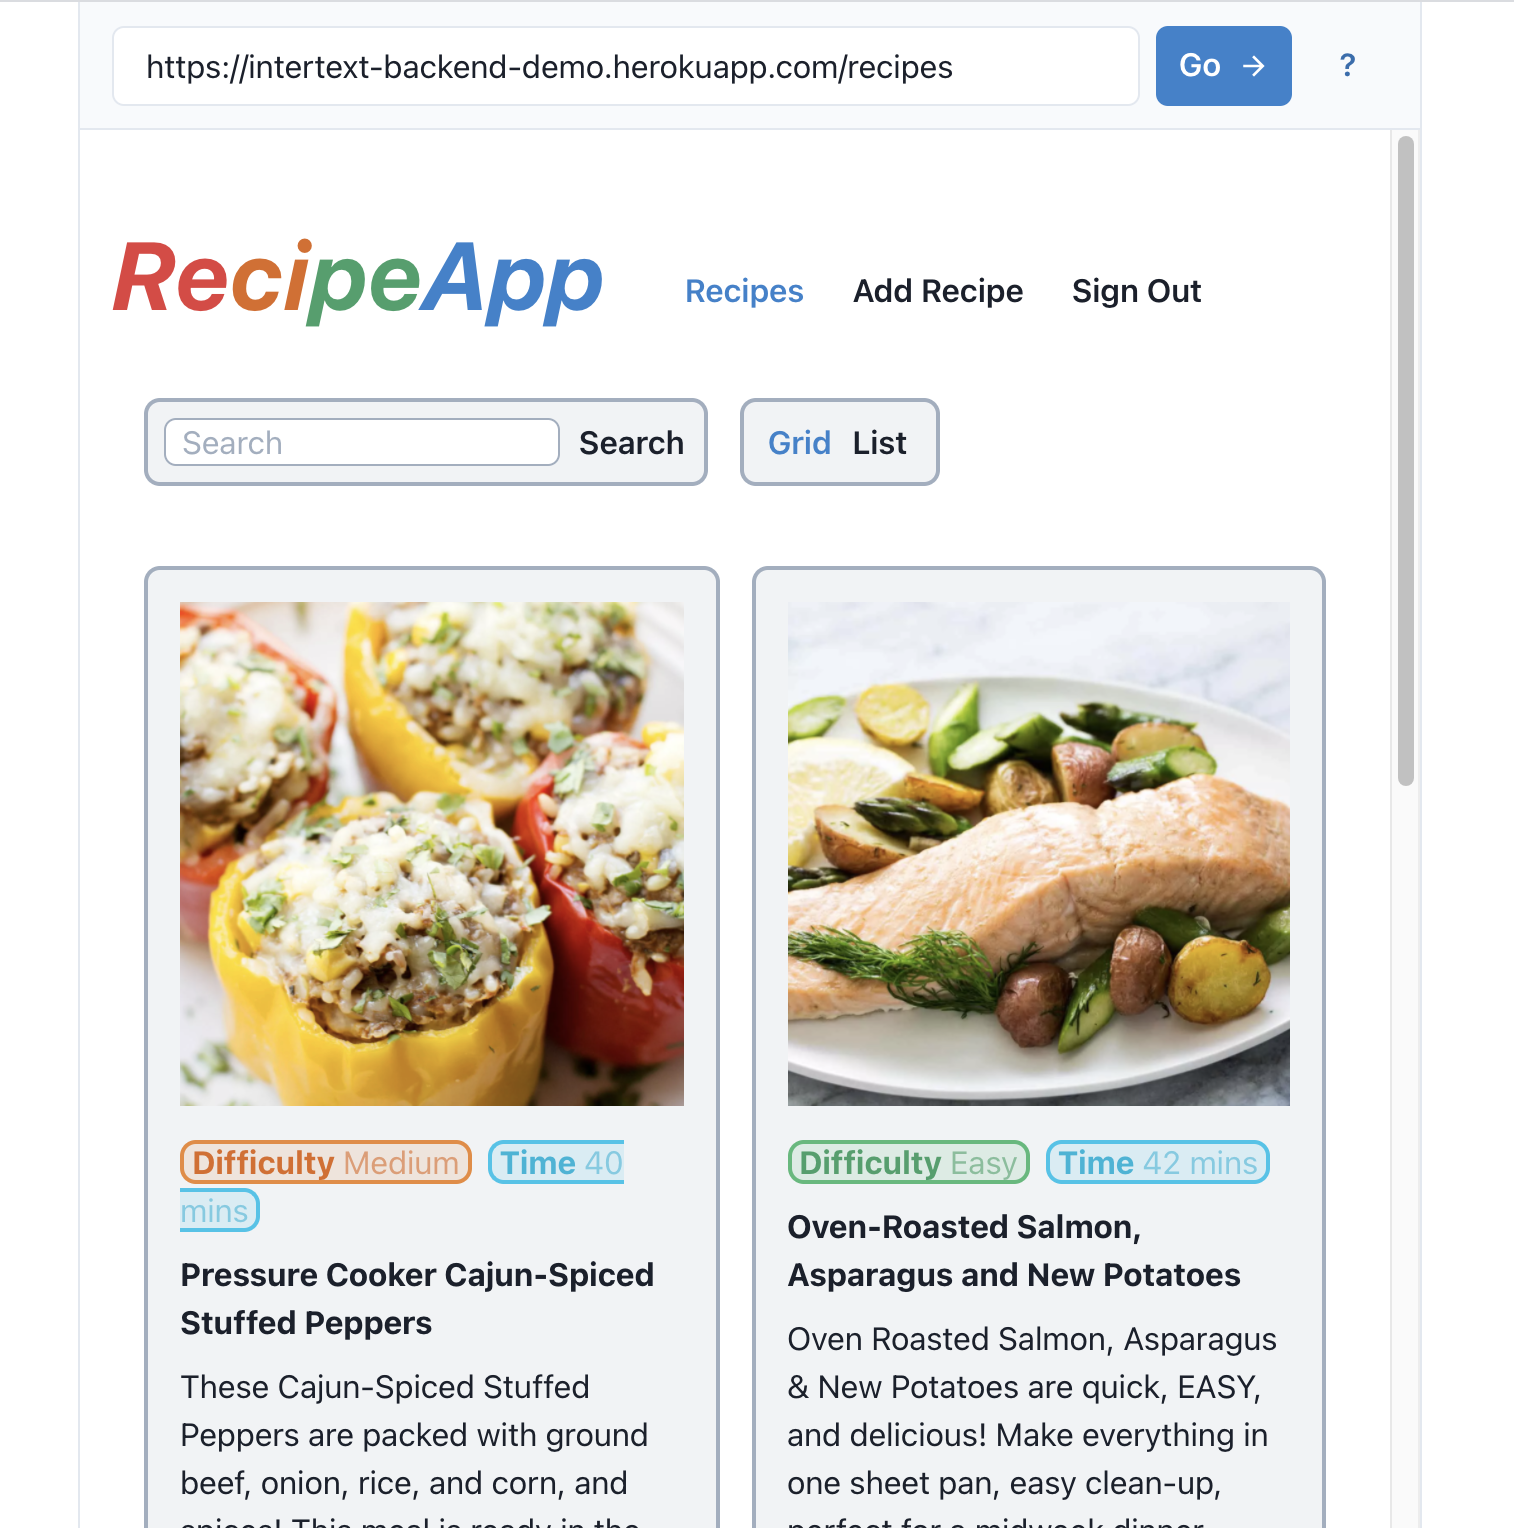
\includegraphics[width=6.2cm]{thesis/paper/images/recipe_grid.png}
  \caption{RecipeApp Recipe List Grid/List Views}%
  \label{fig:rec_recipe_list}%
\end{figure}

Both the input and display preference options work in the same way, by modifying the front-end state and triggering a request to the backend to pick up the modified state. As user types into the text input, Intertext client automatically saves its value into the state that gets passed on to the backend on every request. The \texttt{Search} button next to the search input only triggers a request to the \texttt{/recipes} endpoint. The recipes endpoint receives the query in the search input, and filters the results accordingly. It also pre-populates the input value by passing the query as a children to the \texttt{input} component. The display options on the other hand first sets the front-end state variable \texttt{layout} to either \texttt{grid} or \texttt{list}, and again triggers a request to the same \texttt{recipes} endpoint as seen in Figure~\ref{fig:rec_display_options}. The backend picks up the variable and renders the different version of the displays accordingly. The primary color of the button for the active display option is also controlled by the same \texttt{layout} variable, backend renders the buttons with the relevant intent based on that variable also as seen in Figure~\ref{fig:rec_display_options}.

\begin{figure}[htb]
\begin{minipage}{\linewidth}
\begin{lstlisting}[language=xml]
{{#> button_small}}
  <text intent="{{#if layout_grid}}primary{{else}}{{/if}}">Grid</text>
  <button.onClick>
    <state key="layout" persist="true">grid</state>
    <request endpoint="/recipes"></request>
  </button.onClick>
{{/button_small}}
{{#> button_small}}
  <text intent="{{#if layout_list}}primary{{else}}{{/if}}">List</text>
  <button.onClick>
    <state key="layout" persist="true">list</state>
    <request endpoint="/recipes"></request>
  </button.onClick>
{{/button_small}}
\end{lstlisting}
\end{minipage}
\caption{Redirect screen example}%
\label{fig:rec_display_options}%
\end{figure}


\section{Evaluation}

In this section, we explain how we conducted our user study for user evaluation. We first explain our methodology, and then share the results of our evaluation.

\subsection{Methodology}

We conducted our user study in the form of surveys. We used Google Forms to create the survey and manage the responses. In the surveys, we first gave some information and/or material to investigate, then followed it with Likert scale questions.

We utilised Amazon's Mechanical Turk (MTurk) \footnote{\url{https://www.mturk.com}} service in order to find participants. We stated the description and intentions of each survey on their respective survey page. Some of our surveys required special skills, for which we used features provided by MTurk that enables us to only target participants with special skills. We set the compensation price per answer to 10 cents for general participation surveys, and 50 cents for surveys that requires special skills. We required our participants to enter their \textit{worker id} both on the surveys and on the respective survey page on MTurk, so that we can match the responses of the participants with their MTurk profiles to verify only our intended audience has participated, and duplicate/invalid responses (responses that are submitted without a worker id) are eliminated.

Our user evaluation was conducted in two stages. First stage was to validate the problems in our problem statement that we are intending to solve, and the second stage was to validate Intertext, the solution we offer in order to address these problems. 

\paragraph{Phase 1: Problem Validation}

Here we aimed to validate the problem we are intending to solve. We first asked some optional identifying questions to ask about the background of the participants; including their age, gender, country of origin and occupation. Then, we separated questions into groups for every main category mentioned in our \nameref{problemStatement} section. We directed this section only towards the end users.

\paragraph{Phase 2: Solution Validation}

Our project targets two different user groups; developers, and end users. We created two separate surveys, one for developers and one for end users. On the survey we prepared for the end users, we first gave a brief explanation of what Intertext is and what it does without going into technical details. We told participants about Intertext clients, how it works and how it can be used. We kept it as simple as possible, to make sure the general public can understand it. We also linked to a demo from the Intertext web client. Then, similarly to what we did in the first phase, we stated every problem from the \nameref{problemStatement} section. For every problem, we wrote a short paragraph explaining what the problem exactly is, and one explaining how Intertext addresses that problem. Then, we followed it with Likert scale questions. 

For the developer survey, we started it off by duplicating the one for end users and removing the questions. We kept the information parts identical, as developers also needs to understand what Intertext does and why it is beneficial to the users. We then created an extra section to give a technical overview of how Intertext works, benefits, and how Intertext applications can be developed. We also included a link to the repository that hosts \texttt{RecipeApp}, our demo Intertext application. Next, we listed the developer-related problems from the \nameref{problemStatement} section, wrote a paragraph explaining it, and another paragraph explaining the solution. We followed it with Likert scale questions just like in end user survey format.

In our Likert scale questions, we focused on the trade-offs in order to get answers as objective as possible. To elaborate on this, if we were to explained that we solved a problem, and then followed it with a question asking about the thoughts on the solution, the responses would most certainly be positive. Solving a problem often comes with a trade-off, and this trade-off might not be immediately visible to the participant. We attempted to ask questions in a way that raises an awareness about the trade-offs, and validates if participant is on board with the solution regardless of it. For example, one of the solutions we offer is guaranteed security by eliminating third-party code execution, and the trade-off of this is that the platform will not support rich front-end functionalities and experiences. For general public, this trade-off would likely be overlooked. Thus, the Likert scale question we asked about this solution was \textit{I would prefer guaranteed privacy and security over rich front-end functionality}, validating that users care more about privacy and security than rich front-end functionality.

\subsection{Phase 1 Results}

In the first phase, we received 119 responses (after filtering out duplicate answers and answers with invalid worker ids). In this section we included some of the highlights of our survey; full response data and participant demographics can be found in the \nameref{App:AppendixA}. Our results for the first phase are very positive, we were able to validate the problem and implement Intertext with more confidence.

% ------ ui / ux

\begin{figure}[H]
\centering
\begin{tikzpicture}
\tikzstyle{every node}=[font=\small]

\pie[radius=2,color={green!70,green!30,gray!30,red!40,red!70}]{10.9/,50.4/,28.6/,8.4/,1.7/}

\pie[radius=2,text=legend,pos={4.5,0},color={green!70,green!30,gray!30,red!40,red!70}]{
      16.8/Strongly agree,
      49.6/Agree,
      22.7/Neutral,
      10.1/Disagree,
      0.8/Strongly disagree}

\end{tikzpicture}
\vspace*{-5mm}
\caption{\newline\textit{I experience UI/UX inconsistencies in some applications} (left)\newline\textit{I sometimes experience poor design in some applications} (right)} \label{fig:ev_p1_1}
\end{figure}

Our first two questions focuses on how users perceive applications they use on a daily basis in terms of user experience or user interfaces. We asked participants whether they experience poor design or inconsistent user interfaces/user experiences, and most of them responded by stating that they experience some form of an issue, as it can be seen in figure~\ref{fig:ev_p1_1}.

% ------ ads 

\begin{figure}[H]
\centering
\begin{tikzpicture}
\tikzstyle{every node}=[font=\small]

\pie[radius=2,color={green!70,green!30,gray!30,red!40,red!70}]{12.6/,50.4/,21.0/,10.1/,5.9/}

\pie[radius=2,text=legend,pos={4.5,0},color={green!70,green!30,gray!30,red!40,red!70}]{
      19.3/Strongly agree,
      33.6/Agree,
      21.8/Neutral,
      15.1/Disagree,
      10.1/Strongly disagree}

\end{tikzpicture}
\vspace*{-5mm}
\caption{\newline\textit{Advertisement sector is out of control} (left)\newline\textit{I would rather pay a small fee than seeing ads} (right)} \label{fig:ev_p1_2}
\end{figure}

Next, we focused on advertisement, as it can be seen as one of the leading causes of frustration and a major aspect that hinders user experience for many users. As we expected, there is a strong opinion against advertisement. There seems to be a consensus that the advertisement sector is out of control, and more than 65\% of our participants stated that they use an ad blocking software. In order to understand the extent of the frustration, we asked whether participants would be willing to pay a small fee rather than seeing ads, more than half of our participants responded positively as it can be seen in figure~\ref{fig:ev_p1_2}. Detailed information on the responses related to advertisement can be found in the \nameref{App:AppendixA}.

% ------ customisability

\begin{figure}[H]
\centering
\begin{tikzpicture}
\tikzstyle{every node}=[font=\small]

\pie[radius=2,color={green!70,green!30,gray!30,red!40,red!70}]{16.0/,47.9/,28.6/,6.7/,0.8/}

\pie[radius=2,text=legend,pos={4.5,0},color={green!70,green!30,gray!30,red!40,red!70}]{
      18.5/Strongly agree,
      47.9/Agree,
      22.7/Neutral,
      8.4/Disagree,
      2.5/Strongly disagree}

\end{tikzpicture}
\vspace*{-5mm}
\caption{\newline\textit{I wish I was able to customise the appearances of websites/applications} (left)\newline\textit{I wish I could choose or create a universal theme that would apply to all websites/applications} (right)} \label{fig:ev_p1_3}
\end{figure}

Customisability is another aspect we asked our participants about. While some specific applications, such as code editors allows extensive customisation for their end users, it is not a very common in typical front-end applications. In the recent years, design trends that has been surfacing suggests some level of customisation options are being offered by modern front-end applications, and these changes are often greatly appreciated by many users. For instance, Github recently released a dark mode option and announced this new feature on the Twitter platform \footnote{https://twitter.com/github/status/1336362679506784256}. The extent of support and appreciation can be seen from the responses. However customisability is usually limited to simple adjustments such as the colour theme and font sizes. The responses we received as it can be seen in figure~\ref{fig:ev_p1_3} shows that users are mostly positive about possibilities of extended customisability offerings. Furthermore we asked participants their opinion on a universal theme that would apply to all websites/applications they use, hinting to the unified approach that Intertext adopts, and we received even more positive responses, more than 65\% of our users responded positively.

% ------ cross-platform availability

\begin{figure}[H]
\centering
\begin{tikzpicture}
\tikzstyle{every node}=[font=\small]

\pie[radius=2,color={green!70,green!30,gray!30,red!40,red!70}]{16.0/,60.5/,18.5/,5.0/,0/}

\pie[radius=2,text=legend,pos={4.5,0},color={green!70,green!30,gray!30,red!40,red!70}]{
      36.1/Strongly agree,
      38.7/Agree,
      18.5/Neutral,
      5.9/Disagree,
      0.8/Strongly disagree}

\end{tikzpicture}
\vspace*{-5mm}
\caption{\newline\textit{Applications I use on a daily basis are mostly available on all my devices/platforms} (left)\newline\textit{If I am going to use a service just for once, I prefer using their website instead of downloading their application on my phone} (right)} \label{fig:ev_p1_4}
\end{figure}

Next, we asked about the cross-platform availability of participants daily websites/applications. Most of the participants stated that the applications they use on a daily basis are mostly available on all their devices and platforms. This was a rather unexpected outcome, we concluded that most popular websites/applications used on a daily basis such as internet browsers, email clients, music players, social applications and note taking applications are either already available for popular mobile/desktop platforms and web natively, or they offer some or all of their functionality through an API, allowing replacement applications to be built. We also asked if they go through the inconvenience of downloading an application for services/products that they will be using only once, and the majority of our participants stated that they refrain from downloading the application and prefer using the website in such cases.

% ------ privacy/security

\begin{figure}[H]
\centering
\begin{tikzpicture}
\tikzstyle{every node}=[font=\small]

\pie[radius=2,color={green!70,green!30,gray!30,red!40,red!70}]{39.5/,41.2/,15.1/,4.2/,0/}

\pie[radius=2,text=legend,pos={4.5,0},color={green!70,green!30,gray!30,red!40,red!70}]{
      14.3/Strongly agree,
      49.6/Agree,
      21.8/Neutral,
      10.1/Disagree,
      4.2/Strongly disagree}

\end{tikzpicture}
\vspace*{-5mm}
\caption{\newline\textit{I care about my privacy on the internet} (left)\newline\textit{I would rather pay a small fee than paying with my data} (right)} \label{fig:ev_p1_5}
\end{figure}

Lastly, we asked users opinions on privacy and security. We found that most of the participants do not have major concerns on security, however we noticed a strong stance about online privacy. More than 80\% of our participants stated that they care about their privacy online, and more than 60\% stated that they would rather pay a fee than compromising their privacy.


\subsection{Phase 2 Results}

As mentioned in the previous section, we conducted two separate questionnaire targeting end users and developers for phase two of our user survey. After removing duplicate submissions and responses with invalid worker ids, we were left with 54 submissions for the end users survey, and 14 for the developer survey. Below we present the highlights of both surveys, full response data as well as the participant demographics can be found in the \nameref{App:AppendixA}.

% ------ standardised ui components

\begin{figure}[H]
\centering
\begin{tikzpicture}
\tikzstyle{every node}=[font=\small]

\pie[radius=2,color={green!70,green!30,gray!30,red!40,red!70}]{18.5/,64.8/,13.0/,1.8/,1.9/}

\pie[radius=2,text=legend,pos={4.5,0},color={green!70,green!30,gray!30,red!40,red!70}]{
      37.0/Strongly agree,
      44.4/Agree,
      16.7/Neutral,
      1.9/Disagree,
      0/Strongly disagree}

\end{tikzpicture}
\vspace*{-5mm}
\caption{\textbf{end user survey}\newline\textit{Standardised UI components will improve the consistency across front-end applications} (left)\newline\textit{I prefer consistency over variability} (right)} \label{fig:ev_p2_1}
\end{figure}

First set of questions on the end user survey was on the standardised UI components of Intertext. Participants were extremely positive about this approach, more than 80\% of our participants responded that this will improve the consistency across front-end applications. One drawback of this approach is that there will be less variability, however once again more than 80\% of the participants stated that they prefer consistency over variability, with 37\% of them responding with \texttt{Strongly agree}.

% ------ advertisement

\begin{figure}[H]
\centering
\begin{tikzpicture}
\tikzstyle{every node}=[font=\small]

\pie[radius=2,color={green!70,green!30,gray!30,red!40,red!70}]{29.6/,48.1/,13.0/,7.4/,1.9/}

\pie[radius=2,text=legend,pos={4.5,0},color={green!70,green!30,gray!30,red!40,red!70}]{
      31.5/Strongly agree,
      48.1/Agree,
      14.8/Neutral,
      3.7/Disagree,
      1.9/Strongly disagree}

\end{tikzpicture}
\vspace*{-5mm}
\caption{\textbf{end user survey}\newline\textit{I prefer advertisements to blend in naturally to the look-and-feel of the website instead of sticking out} (left)\newline\textit{I am okay with seeing non-intrusive and respectful advertisement (with no compromise of privacy), OR paying a small fee in order to support the creator} (right)} \label{fig:ev_p2_2}
\end{figure}

Then, we asked about the implications of Intertext on advertisement. Intertext prevents online advertisers to create ads that are intrusive that hinder user experience. Intertext however cannot and does not prevent advertisements in general, but enforces them to be respectful to the user in terms of user experience and privacy. Most of our participants felt positive about this, they stated that they would prefer advertisements to blend in naturally with the website rather sticking out. They were even supportive of this as most of them stated that they were okay with seeing advertisements with respectful boundaries, or paying a small fee, in order to support the content creator.

% ------ accessibility

\begin{figure}[H]
\centering
\begin{tikzpicture}
\tikzstyle{every node}=[font=\small]

\pie[radius=2.5,text=legend,pos={4.5,0},color={green!70,green!30,gray!30,red!40,red!70}]{
      18.5/Strongly agree,
      59.3/Agree,
      18.5/Neutral,
      3.7/Disagree,
      0/Strongly disagree}

\end{tikzpicture}
\vspace*{-1mm}
\caption{\textbf{end user survey}\newline\textit{I would benefit from the guaranteed accessibility aspect of Intertext}} \label{fig:ev_p2_3}
\end{figure}

Next, we had a question on accessibility. Intertext provides components out-of-the-box, all of which are implemented in an accessible way. Thus, Intertext applications that are made out of these components will surely be accessible. For this question, we had a paragraph clarifying to the scope of accessibility; that accessibility is not only for people with disabilities, but how and why in can benefit everyone \footnote{https://www.w3.org/standards/webdesign/accessibility}. Then we asked whether they would personally benefit from Intertext in terms of accessibility perspective, and most of the participants stated that they would.

% ------ customisability

\begin{figure}[H]
\centering
\begin{tikzpicture}
\tikzstyle{every node}=[font=\small]

\pie[radius=2,color={green!70,green!30,gray!30,red!40,red!70}]{37.0/,44.4/,16.7/,1.9/,0/}

\pie[radius=2,text=legend,pos={4.5,0},color={green!70,green!30,gray!30,red!40,red!70}]{
      29.6/Strongly agree,
      61.1/Agree,
      7.4/Neutral,
      1.9/Disagree,
      0/Strongly disagree}

\end{tikzpicture}
\vspace*{-5mm}
\caption{\textbf{end user survey}\newline\textit{I prefer customisability over variability} (left)\newline\textit{I love that I can create my own theme OR chose a theme I like that applies for all applications} (right)} \label{fig:ev_p2_4}
\end{figure}

We found after our user studies that customisability is one of the aspects that gets the most support and positivity. In this phase of our study, most of our participants responded very positively to our questions regarding customisability. One drawback of customisability is the necessity of standardised component approach, which impacts variability of user interfaces across applications. However our studies suggest that this does not bother users at all, most of our users were in favour of customisability at the cost of variability. In fact, more than 90\% of our users responded that they would love it if they can choose a universal theme that applies to all front-ends across applications.

% ------ cross platform support

\begin{figure}[H]
\centering
\begin{tikzpicture}
\tikzstyle{every node}=[font=\small]

\pie[radius=2,color={green!70,green!30,gray!30,red!40,red!70}]{33.3/,53.7/,7.4/,5.6/,0/}

\pie[radius=2,text=legend,pos={4.5,0},color={green!70,green!30,gray!30,red!40,red!70}]{
      37.0/Strongly agree,
      46.3/Agree,
      11.1/Neutral,
      1.9/Disagree,
      3.7/Strongly disagree}

\end{tikzpicture}
\vspace*{-5mm}
\caption{\textbf{end user survey}\newline\textit{I would be interested in seeing applications running natively on alternative platforms/devices (other than desktop/mobile; such as wearables, command-line interfaces and so on)} (left)\newline\textit{If all devices/platforms/environments supported all applications that I use natively, it would increase the use of my other devices} (right)} \label{fig:ev_p2_5}
\end{figure}

Responses to questions regarding the cross-platform support came rather unexpectedly. Our study from phase 1 suggested that participants were not overly enthusiastic about cross-platform availability as most of their daily applications were already supported on their devices, and they did not seem to have a notable issue with lack of cross-platform support. However, once they were introduced to Intertext and the cross-platform support that comes with it, it appeared that participants were largely in favour of said support, especially on alternative devices rather than traditional desktop/mobile platforms. Most of the participants stated that they would be interested in seeing applications running natively on non-traditional devices/platforms such as wearables and command-line interfaces. They also stated that if this was the case, it would likely increase their usage of alternative devices/platforms.

% ------ privacy/security

\begin{figure}[H]
\centering
\begin{tikzpicture}
\tikzstyle{every node}=[font=\small]

\pie[radius=2,text=legend,pos={4.5,0},color={green!70,green!30,gray!30,red!40,red!70}]{
      25.9/Strongly agree,
      64.8/Agree,
      3.7/Neutral,
      5.6/Disagree,
      0/Strongly disagree}

\end{tikzpicture}
\vspace*{-1mm}
\caption{\textbf{end user survey}\newline\textit{I would prefer guaranteed privacy and security over rich front-end functionality}} \label{fig:ev_p2_6}
\end{figure}

Intertext guarantees security/privacy by preventing third-party code execution on users devices. This is achieved by forcing developers to implement business logic on the server side, and only accepting non-executable XML code that renders on user device by an Intertext client. The obvious drawback of this approach is the possibility of building applications with rich front-end functionality. We asked participants opinion on this matter, and most of the participants stated that they would prefer privacy/security over said front-end functionalities.

% ------ developer

\begin{figure}[H]
\centering
\begin{tikzpicture}
\tikzstyle{every node}=[font=\small]

\pie[radius=2,color={green!70,green!30,gray!30,red!40,red!70}]{28.6/,42.9/,28.6/,0/,0/}

\pie[radius=2,text=legend,pos={4.5,0},color={green!70,green!30,gray!30,red!40,red!70}]{
      7.1/Strongly agree,
      57.1/Agree,
      35.7/Neutral,
      0/Disagree,
      0/Strongly disagree}

\pie[radius=2,pos={2.25,3.9},color={green!70,green!30,gray!30,red!40,red!70}]{35.7/,50.0/,14.3/,0/,0/}

\end{tikzpicture}
\vspace*{-1mm}
\caption{\textbf{developer survey}\newline\textit{I would prefer using IUIDL over building my own components from scratch with the cost of:}
\newline- \textit{adding cross-platform support} (top)
\newline- \textit{making them accessible} (left)
\newline- \textit{maintenance} (right)} \label{fig:ev_p2_7}
\end{figure}

As for the developer survey, we received a mix of positive and neutral responses. In this survey, we gave an overall rundown of Intertext and provided a technical overview with a demo codebase. Then we asked developers whether or not they would prefer using Intertext for benefits in cross-platform support, accessibility and maintenance. In all three categories the responses were mostly positive as seen in figure~\ref{fig:ev_p2_7}.